\documentclass[ignorenonframetext,]{beamer}
\setbeamertemplate{caption}[numbered]
\setbeamertemplate{caption label separator}{: }
\setbeamercolor{caption name}{fg=normal text.fg}
\beamertemplatenavigationsymbolsempty
\usepackage{lmodern}
\usepackage{amssymb,amsmath}
\usepackage{ifxetex,ifluatex}
\usepackage{fixltx2e} % provides \textsubscript
\ifnum 0\ifxetex 1\fi\ifluatex 1\fi=0 % if pdftex
\usepackage[T1]{fontenc}
\usepackage[utf8]{inputenc}
\else % if luatex or xelatex
\ifxetex
\usepackage{mathspec}
\else
\usepackage{fontspec}
\fi
\defaultfontfeatures{Ligatures=TeX,Scale=MatchLowercase}
\fi
% use upquote if available, for straight quotes in verbatim environments
\IfFileExists{upquote.sty}{\usepackage{upquote}}{}
% use microtype if available
\IfFileExists{microtype.sty}{%
\usepackage{microtype}
\UseMicrotypeSet[protrusion]{basicmath} % disable protrusion for tt fonts
}{}
\newif\ifbibliography

% Prevent slide breaks in the middle of a paragraph:
\widowpenalties 1 10000
\raggedbottom

\AtBeginPart{
\let\insertpartnumber\relax
\let\partname\relax
\frame{\partpage}
}
\AtBeginSection{
\ifbibliography
\else
\let\insertsectionnumber\relax
\let\sectionname\relax
\frame{\sectionpage}
\fi
}
\AtBeginSubsection{
\let\insertsubsectionnumber\relax
\let\subsectionname\relax
\frame{\subsectionpage}
}

\setlength{\parindent}{0pt}
\setlength{\parskip}{6pt plus 2pt minus 1pt}
\setlength{\emergencystretch}{3em}  % prevent overfull lines
\providecommand{\tightlist}{%
\setlength{\itemsep}{0pt}\setlength{\parskip}{0pt}}
\setcounter{secnumdepth}{0}

\title{STA305/1004 - Class 5}
\date{January 23, 2017}

\begin{document}
\frame{\titlepage}

\begin{frame}{Today's Class}

\begin{itemize}
\tightlist
\item
  REMINDER: Assignment \#1 due Jan. 27 on Crowdmark via portal by 22:00
\item
  In-class problem on last week's material
\item
  Introduction to Phase III Clinical Trials
\item
  Introduction to power
\end{itemize}

\end{frame}

\begin{frame}{What are clinical trials?}

Clinical trials are prospective intervention studies with human subjects
to investigate experimental drugs, new treatments, medical devices, or
clinical procedures (Yin, 2012).

\end{frame}

\begin{frame}{Phases of clinical trials}

Developing a new drug for cancer.

\begin{itemize}
\item
  \textbf{Preclinical studies:} In vitro (e.g.~slides, test tubes) and
  in vivo (living organism such as rodents) studies on wide range of
  doses of experimental agents. This stage of study provides preliminary
  toxicity and efficacy data including pharmacokinetics (PK) and
  pharmacodynamics (PD) information.
\item
  \textbf{Phase I:} Usually first study in humans to investigate the
  toxicity and side effects of the new agent. Identify MTD.
\item
  \textbf{Phase II:} Assess if drug has sufficient efficacy. The drug is
  usually administered around the MTD. If drug does not show efficacy or
  is too toxic then further testing is discontinued.
\end{itemize}

\end{frame}

\begin{frame}{Phases of clinical trials}

\begin{itemize}
\item
  \textbf{Phase III:} If drug passes phase II testing then it is
  compared to the current standard of care or placebo. These are
  long-term, large scale randomized studies that may involve hundreds or
  thousands of patients.
\item
  If the drug is proven to be effective (e.g.~two positive phase III
  trials required for FDA approval) the company will file an application
  with regulatory agencies to sell the drug. If approved then the drug
  will be available to the general population in the country where it
  was approved.
\item
  \textbf{Phase IV:} After approval a study might follow a large number
  of patients over a longer period of time to monitor side effects and
  drug interactions. For example, findings from these studies might add
  a warning label to the drug.
\end{itemize}

\end{frame}

\begin{frame}{Phases of clinical trials}

\begin{itemize}
\tightlist
\item
  The four phases are usually conducted sequentially and separately.
\item
  Each trial requires an independent study design and a study protocol.
\item
  Every aspect of trial design, monitoring, and data analysis call upon
  statistical methods.
\item
  In randomized clinical trials a treatment group is often referred to
  as an \textbf{arm}.
\end{itemize}

\end{frame}

\begin{frame}{Phases of clinical trials}

\begin{itemize}
\item
  Experimental design plays a very important role in the design of
  clinical trials.
\item
  Two arm clinical trials use all of theory of randomization that we
  learned about last week. Randomization is used to design phase III
  clinical trials since causation can usually be assessed using a
  randomized design.
\end{itemize}

\end{frame}

\begin{frame}{How can causation be assessed using a randomized design?}

\begin{itemize}
\item
  Suppose that patients are randomized in a two arm clinical trial where
  one of the arms is the standard treatment and the other arm is an
  experimental treatment
\item
  A statistically significant difference in the outcome between the two
  arms is observed showing the experimental treatment is more
  efficacious.
\item
  The interpretation is that the experimental treatment \emph{caused}
  patients to have a better outcome since the only difference between
  the two arms is the treatment. Randomization is supposed to ensure
  that the groups will be similar with respect to all the factors
  measured in the study and all the factors that are not measured.
\end{itemize}

\end{frame}

\begin{frame}{How can causation be assessed using a randomized design?}


\includegraphics[width=10cm, height=8cm]{nejm1.png}

\end{frame}

\begin{frame}{How can causation be assessed using a randomized design?}

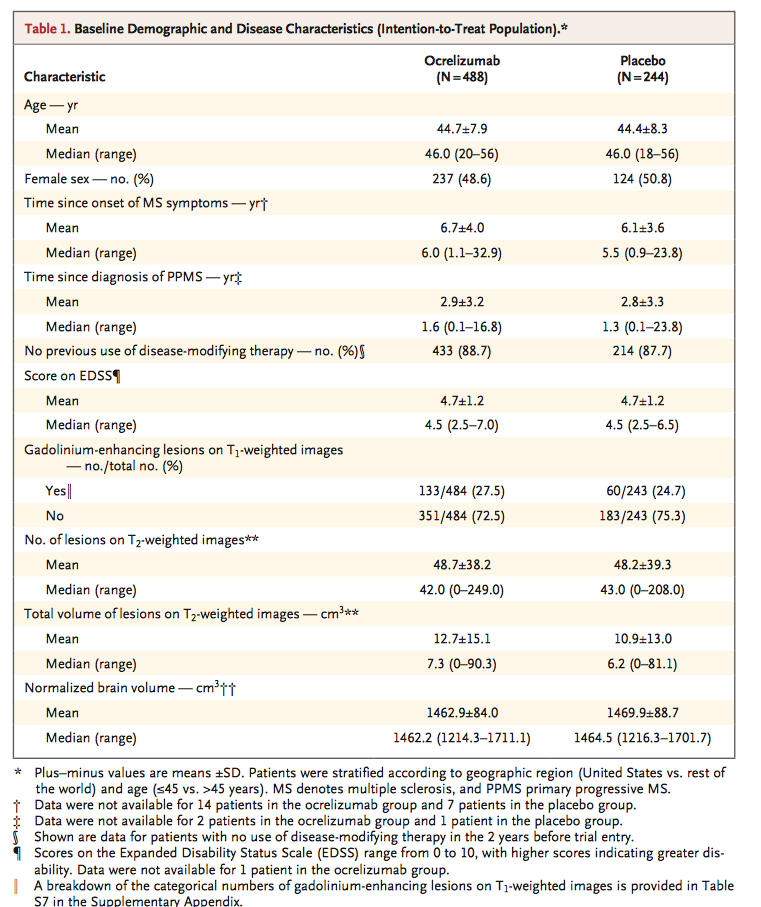
\includegraphics[width=10cm, height=8cm]{nejm2.png}

\end{frame}

\begin{frame}{How many patients should be enrolled in a Phase III
clinical trial?}

\begin{itemize}
\tightlist
\item
  In a phase III trial sample size is the most critical component of the
  study design. The sample size has implications for how many subjects
  will be exposed to a drug that has no proven efficacy.
\item
  The investigator needs to specify type I, II error rates, and the
  effect sizes.
\item
  Standard practice is to compute the smallest sample size required to
  detect a clinically important/significant treatment difference with
  sufficient.
\end{itemize}

\end{frame}

\begin{frame}{How many patients should be enrolled in a Phase III
clinical trial?}

\begin{itemize}
\tightlist
\item
  If the sample size is too small then the trial might fail to discover
  a truly effective drug because the statistical test cannot reach the
  significance level (5\%) due to a lack of power.
\item
  If the sample size is overestimated then resources wasted and drug
  development delayed since patient enrollment is often the main factor
  in time to complete a trial.
\end{itemize}

\end{frame}

\begin{frame}{Statistical hypotheses}

Suppose that subjects are randomized to treatments A or B with equal
probability. Let \(\mu_A\) be the mean response in the group receiving
drug A and \(\mu_B\) be the mean response in the group receiving drug B.
The null hypothesis is that there is no difference between A and B, the
alternative claims there is a clinically meaningful difference between
them.

\[H_0:\mu_A=\mu_B \thinspace \text{ versus } \thinspace H_0:\mu_A \ne \mu_B \]

\end{frame}

\begin{frame}{Statistical hypotheses}

The type I error rate is defined as:

\[\begin{aligned}
\alpha &=P\left(\text{type I error}\right) \\
       &=P\left(\text{Reject } H_0 \text{ when }H_0 \text{ is true}\right).\\
\end{aligned}\]

\end{frame}

\begin{frame}{Statistical hypotheses}

The type II error rate is defined as:

\[\begin{aligned}
\beta&=P\left(\text{type II error}\right) \\
     &=P\left(\text{Accept }H_0 \text{ when }H_1 \text{ is true}\right).   
\end{aligned}\]

\end{frame}

\begin{frame}{Statistical hypotheses}

Power is define as: \[ \begin{aligned}
\text {power} &= 1-\beta \\
              &= 1-P\left(\text{Accept }H_0 \text{ when }H_1 \text{ is true}\right) \\
              &= P\left(\text{Reject } H_0 \text{ when }H_1 \text{ is true}\right).
\end{aligned}\]

\end{frame}

\begin{frame}{Power}

The probability that a fixed level \(\alpha\) test will reject \(H_0\)
when a particular alternative value of the parameter is true is called
power of the test to detect that alternative.

\end{frame}

\begin{frame}{Power}

Can a 6-month exercise program increase the total body bone mineral
content (TBBMC) of young women? Based on results of a previous study
\(\sigma=2\) for the percent change in TBBMC over the 6-month period. A
change in TBBMC of 1\% would be considered important. Is 25 subjects a
large enough sample size for this project?

\end{frame}

\end{document}
